\documentclass[aspectratio=169, table]{beamer}

\usepackage{colortbl}
\usepackage{xcolor}
\usepackage{listings}
\usepackage{tikz}
\usepackage{pgfplots}
\usepgfplotslibrary{polar}
\usetikzlibrary{arrows.meta, positioning, calc}

\usetheme{Pradita}


\usepackage{listings}
\lstdefinestyle{SqlStyle}{
language=SQL,
basicstyle=\ttfamily\footnotesize,
morekeywords={REAL, TEXT, REFERENCES},
keywordstyle=\color{blue},
commentstyle=\color{gray},
stringstyle=\color{red},
breaklines=true,
showstringspaces=false,
tabsize=2,
captionpos=b,
numbers=left,
numberstyle=\tiny\color{gray},
frame=lines,
backgroundcolor=\color{lightgray!10},
comment=[l]{//},
morecomment=[s]{/*}{*/},
commentstyle=\color{gray}\ttfamily,
string=[s]{'}{'},
morestring=[s]{"}{"},
%	stringstyle=\color{teal}\ttfamily,
%	showstringspaces=false
}

\lstdefinelanguage{bash} {
keywords={},
basicstyle=\ttfamily\small,
keywordstyle=\color{blue}\bfseries,
ndkeywords={iex},
ndkeywordstyle=\color{purple}\bfseries,
sensitive=true,
commentstyle=\color{gray},
stringstyle=\color{red},
numbers=left,
numberstyle=\tiny\color{gray},
breaklines=true,
frame=lines,
backgroundcolor=\color{lightgray!10},
tabsize=2,
comment=[l]{\#},
morecomment=[s]{/*}{*/},
commentstyle=\color{gray}\ttfamily,
stringstyle=\color{purple}\ttfamily,
showstringspaces=false
}

% Define Java language style for listings
\lstdefinestyle{JavaScript}{
	language=Java,
	basicstyle=\ttfamily\footnotesize,
	keywordstyle=\color{blue},
	commentstyle=\color{gray},
	stringstyle=\color{red},
	breaklines=true,
	showstringspaces=false,
	tabsize=4,
	captionpos=b,
	numbers=left,
	numberstyle=\tiny\color{gray},
	frame=lines,
	backgroundcolor=\color{lightgray!10},
	comment=[l]{//},
	morecomment=[s]{/*}{*/},
	commentstyle=\color{gray}\ttfamily,
	string=[s]{'}{'},
	morestring=[s]{"}{"},
	%	stringstyle=\color{teal}\ttfamily,
	%	showstringspaces=false
}

\title{\Huge Business Intelligence \\
\vspace{10pt}
and Dashboards}
\subtitle{IT140704 - Big Data for Business}
%\date[Serial]{Penggunaan Large Language Model untuk Pengajaran}
\author{\textbf{Alfa Yohannis}}
\begin{document}

\frame{\titlepage}


\begin{frame}[fragile]
\frametitle{Contents}
\vspace{20pt}
\begin{columns}[t]
	\column{0.5\textwidth}
	\tableofcontents[sections={1-5}]
	
	\column{0.5\textwidth}
	\tableofcontents[sections={6-20}]
\end{columns}
\end{frame}

\begin{frame}{\hfill}
	\centering
	\Huge{\textbf{How can data be used to create real strategic, tactical, and operational values?}}
\end{frame}


\section{Introduction to Business Intelligence}


\begin{frame}{Dashboards}
	\vspace{20pt}
	\centering
	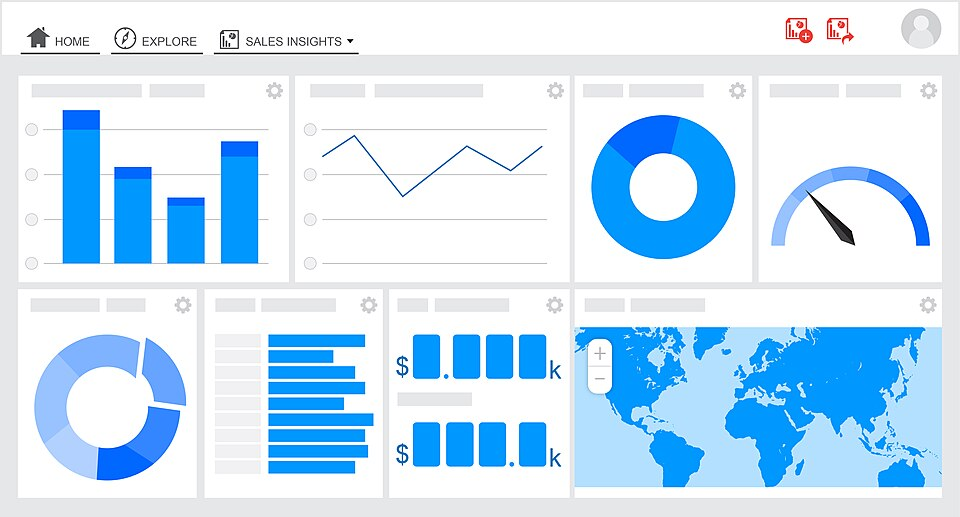
\includegraphics[width=0.9\textwidth]{figures/dashboard.jpg}
\end{frame}


\begin{frame}{Data Warehouse and Data Mart}
	\vspace{20pt}
	\centering
	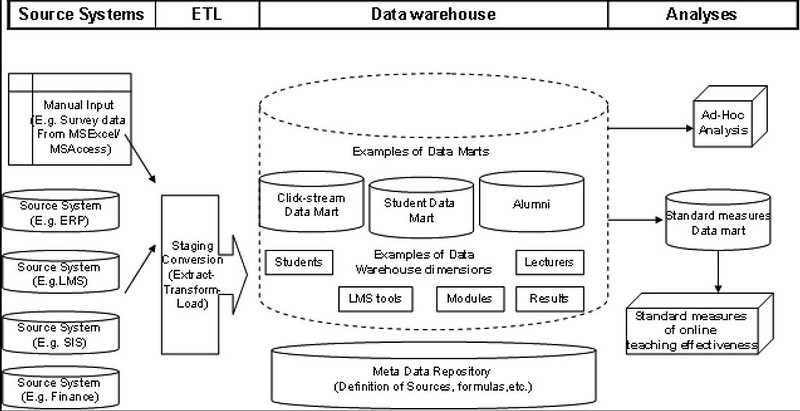
\includegraphics[width=0.9\textwidth]{figures/datamart.jpg}
\end{frame}


\begin{frame}{Introduction to Business Intelligence}
	\vspace{20pt}
	\begin{itemize}
		\item \textbf{Data-Driven Shift.} Digital transformation replaces intuition with data-based decisions.
		\item \textbf{BI Capabilities.} Transforms raw data into insights through ETL and visualisation.
		\item \textbf{Broad Usage.} Adopted by both large companies and SMEs.
		\item \textbf{Key Components.} Covers architecture, visualisation, and tools like Power BI/Tableau.
		\item \textbf{Managerial Access.} Dashboards allow insights without coding knowledge.
		\item \textbf{Strategic Value.} Enables KPI tracking, trend analysis, and anomaly detection.
	\end{itemize}
\end{frame}

\section{Core Concepts of Business Intelligence}

\begin{frame}{Core Concepts of Business Intelligence}
	\vspace{20pt}
	\begin{itemize}
		\item \textbf{Definition.} BI is a set of processes, architecture, and technologies that transform raw data into actionable information.
		\item \textbf{Key Components.} Includes ETL (Extract, Transform, Load), data warehousing, OLAP, data mining, and reporting tools.
		\item \textbf{Decision Support.} Enables strategic, tactical, and operational decision-making based on evidence, not intuition.
		\item \textbf{Business Impact.} Helps organisations detect hidden patterns, monitor KPIs, and respond to market changes.
		\item \textbf{BI vs Big Data.} BI handles structured internal data, including the visualization; Big Data deals with large, fast, varied data using advanced technologies.
	\end{itemize}
\end{frame}

\section{Business Intelligence Architecture}

\begin{frame}{Data Sources and ETL in BI Architecture}
	\vspace{20pt}
	\begin{itemize}
		\item \textbf{Data Sources.} BI relies on internal systems (ERP, CRM, POS), spreadsheets, and external sources like social media or financial data.
		\item \textbf{ETL Process.} Involves Extracting data, Transforming it to standard formats, and Loading it into a data warehouse.
		\item \textbf{Data Quality.} ETL ensures consistency, removes duplicates, and handles missing values for reliable analysis.
		\item \textbf{Tools and Trends.} Automation via Talend, Informatica, or Apache NiFi; modern ELT used in cloud and data lake environments.
	\end{itemize}
\end{frame}



\begin{frame}{Data Warehouse and Data Mart}
	\vspace{20pt}
	\begin{itemize}
		\item \textbf{Data Warehouse.} Centralised, historical, cleaned data store for multidimensional analysis and strategic reporting.
		\item \textbf{Schemas.} Typically structured using star or snowflake schemas for exploring data by dimensions like time and region.
		\item \textbf{Data Mart.} Subset of a data warehouse, focused on specific departments (e.g. marketing, finance).
		\item \textbf{Use Case – Telco.} Marketing team uses a campaign-focused data mart built from a broader customer data warehouse.
		\item \textbf{Use Case – University.} Academic units analyse GPA trends from a learning performance data mart derived from a university data warehouse.
	\end{itemize}
\end{frame}

\begin{frame}{OLAP and Multidimensional Cubes}
	\vspace{20pt}
	\begin{itemize}
		\item \textbf{OLAP (Online Analytical Processing).} Enables fast exploration of multidimensional data for trend analysis and strategic decisions.
		\item \textbf{Cube Structure.} Organises data into dimensions (e.g. Time, Region, Product) with measures (e.g. Sales, GPA) stored in cells.
		\item \textbf{Typical Operations.} Includes slicing (filtering by one dimension), dicing (subsetting), drilling down (detail), and rolling up (aggregation).
		\item \textbf{Use Case – Retail.} Analysts slice the cube by month and region to find top-performing products.
		\item \textbf{Use Case – Education.} Faculty drills down from university-wide GPA to department and cohort level.
	\end{itemize}
\end{frame}


\begin{frame}{OLAP Cube Structure}
	\vspace{20pt}
	\centering
	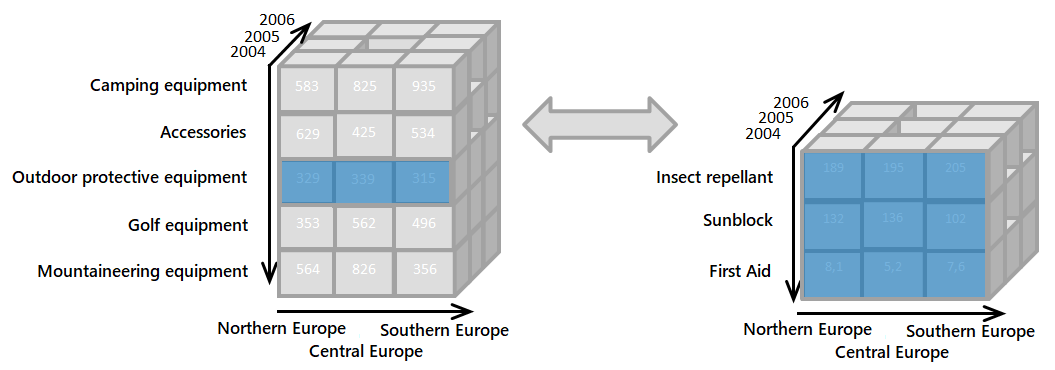
\includegraphics[width=\textwidth]{figures/olap_structure.png}
\end{frame}

\begin{frame}{OLAP Cube Operations}
	\vspace{20pt}
	\centering
	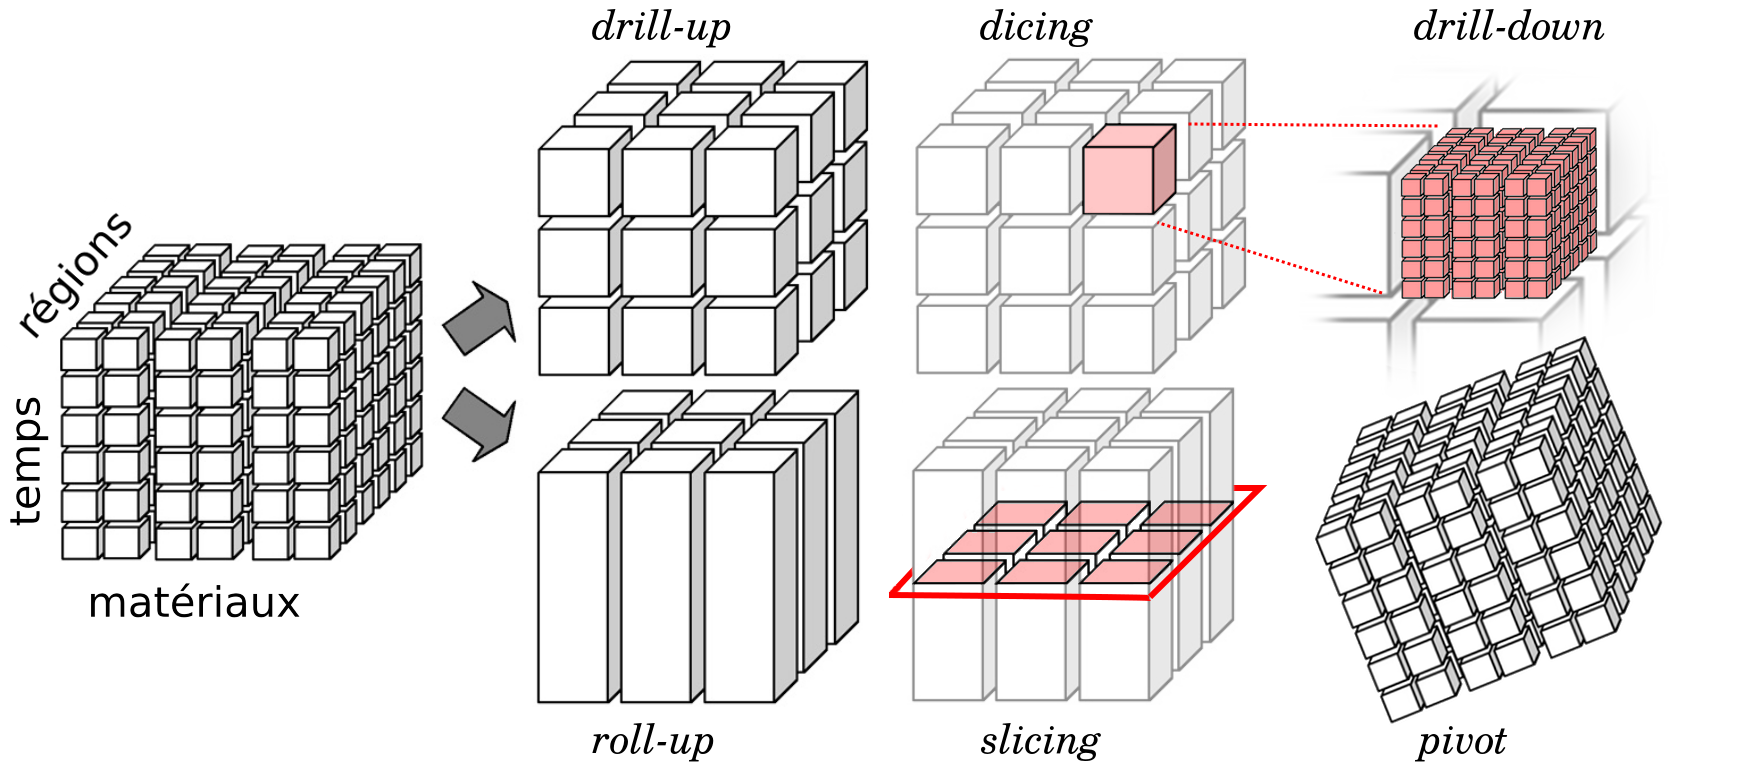
\includegraphics[width=\textwidth]{figures/olap_operations.png}
\end{frame}

\section{Data Visualisation and Dashboards}

\begin{frame}{Effective Data Visualisation Principles}
	\vspace{20pt}
	\begin{itemize}
		\item \textbf{Purpose.} Visualisation bridges complex data and fast decision-making in BI.
		\item \textbf{Clarity.} Effective visuals emphasise clarity, readability, consistency, and relevance.
		\item \textbf{Chart Selection.} Match chart type to data: bar for categories, line for trends, heatmap for correlations.
		\item \textbf{Colour Usage.} Use bright colours to highlight, neutral tones for background.
		\item \textbf{Avoid Clutter.} Minimise 3D effects, animation, and excessive labels to reduce misinterpretation.
	\end{itemize}
\end{frame}


\begin{frame}{Types of Dashboards in BI}
	\vspace{20pt}
	\begin{itemize}
		\item \textbf{Strategic Dashboard.} Used by executives to monitor high-level KPIs like revenue growth or market share; updated weekly or monthly.
		\item \textbf{Tactical Dashboard.} Used by middle managers to evaluate departmental performance and campaign ROI; more analytical in nature.
		\item \textbf{Operational Dashboard.} Supports real-time monitoring by frontline staff or supervisors; tracks daily tasks like deliveries and stock status.
	\end{itemize}
\end{frame}



\begin{frame}{Dashboard Components and Best Practices}
	\vspace{20pt}
	\begin{itemize}
		\item \textbf{Core Elements.} Include clear titles, KPI cards, targeted charts, filters, and narrative notes.
		\item \textbf{User Focus.} Highlight key insights and prompt user action through visual emphasis.
		\item \textbf{Design Principles.} Use one-screen view, top-left prioritisation, limited colours, and interactive filters.
		\item \textbf{User Fit.} Adapt layout for executives (summary-focused) or analysts (explorative).
		\item \textbf{Example.} A support dashboard shows real-time queue load, agent performance, and weekly customer satisfaction trends.
	\end{itemize}
\end{frame}

\section{BI Technology and Tools}


\begin{frame}{Popular BI Tools Overview}
	\vspace{20pt}
	\begin{itemize}
		\item \textbf{Tool Variety.} Popular BI tools include Power BI, Tableau, Qlik Sense, and Google Looker.
		\item \textbf{Power BI.} Integrates with Microsoft ecosystem, supports drag-and-drop dashboards and auto-refresh.
		\item \textbf{Tableau.} Excels in advanced visualisation and interactive data exploration.
		\item \textbf{Qlik Sense.} Uses associative model to explore data without explicit queries.
		\item \textbf{Looker.} Cloud-native, uses LookML to model and query data effectively.
	\end{itemize}
\end{frame}

%\begin{frame}{Criteria for Selecting BI Tools}
%	\vspace{20pt}
%	\begin{itemize}
%		\item \textbf{Key Factors.} Usability, data integration, visualisation flexibility, security, and cost efficiency.
%		\item \textbf{Collaboration Features.} Real-time updates, interactive dashboards, and access control support.
%		\item \textbf{User Type.} Intuitive tools suit non-technical users; scripting and big data support suit analysts and IT teams.
%		\item \textbf{Use Case Example.} A university selects Power BI for affordability; a consultancy prefers Tableau for visual storytelling.
%	\end{itemize}
%\end{frame}



%\begin{frame}{BI Integration with Management Systems}
%	\vspace{20pt}
%	\begin{itemize}
%		\item \textbf{Integration Scope.} Connects BI with ERP, CRM, HRIS, and financial systems for real-time data flow.
%		\item \textbf{Decision Support.} Reduces manual data handling and accelerates decision-making.
%		\item \textbf{Example.} Power BI integrates with Dynamics 365; Tableau connects to Salesforce for sales and customer insights.
%		\item \textbf{Tools.} Use pre-built connectors, APIs, or middleware like Talend and Apache NiFi for ETL processes.
%		\item \textbf{Impact.} Ensures consistent, accurate, and timely information across business units.
%	\end{itemize}
%\end{frame}




\section{Case Studies and BI Implementation}

\begin{frame}{Business Intelligence Use Cases}
	\vspace{20pt}
	\begin{itemize}
		\item \textbf{Retail.} Walmart uses BI to analyse shopping patterns by location, time, and season to optimise stock and promotions.
		\item \textbf{Banking.} BI supports fraud detection, customer segmentation, and accurate credit scoring.
		\item \textbf{Higher Education.} An Indonesian university uses Power BI to track GPA, retention, and LMS activity across programmes.
		\item \textbf{Cross-Sector Adoption.} BI is applied in public services, healthcare, education, and SMEs to enhance decision-making.
	\end{itemize}
\end{frame}


\begin{frame}{Steps for Implementing BI}
	\vspace{20pt}
	\begin{enumerate}
		\item \textbf{Identify Business Needs.} Define problems and strategic information requirements.
		\item \textbf{Select BI Tools.} Match platform features with technical skills and budget.
		\item \textbf{Data Integration (ETL).} Extract, clean, and consolidate data from systems like ERP or CRM.
		\item \textbf{Develop Data Warehouse/Marts.} Build centralised and department-specific repositories.
		\item \textbf{Design Dashboards.} Align visualisations with user roles and KPIs.
		\item \textbf{User Training and Adoption.} Conduct training and refine dashboards based on feedback.
	\end{enumerate}
\end{frame}



\begin{frame}{BI Impl: Challenges and Success Factors}
	\vspace{20pt}
	\begin{itemize}
		\item \textbf{Common Challenges.} Poor data quality, low data literacy, complex integration, weak IT infrastructure, and lack of strategic alignment.
		\item \textbf{Success Factors.} Executive commitment, IT-business collaboration, iterative dashboard development, and accessible, clean data.
		\item \textbf{Case Example.} A logistics firm succeeded by forming a cross-functional agile team focused on delivery timeliness and cost efficiency.
	\end{itemize}
\end{frame}

\section{Ethics and Security in BI}


\begin{frame}{Data Privacy and Access Control}
	\vspace{20pt}
	\begin{itemize}
		\item \textbf{Sensitive Data.} BI often processes personal, financial, or employee data requiring strong privacy safeguards.
		\item \textbf{Privacy Principles.} Apply data minimisation, purpose limitation, and pseudonymisation where possible.
		\item \textbf{Access Control.} Use role-based access to limit visibility of sensitive details to authorised users only.
		\item \textbf{Example.} Employee performance dashboards should show aggregated data, not individual names, to unauthorised viewers.
	\end{itemize}
\end{frame}



\begin{frame}{System Security in BI}
	\vspace{20pt}
	\begin{itemize}
		\item \textbf{Vulnerabilities.} BI systems are exposed to cyber risks due to multiple data sources and web access.
		\item \textbf{Security Measures.} Implement user authentication, role-based authorisation, encryption, and audit logs.
		\item \textbf{Cloud Considerations.} Understand shared responsibility for data protection in cloud-based BI platforms.
		\item \textbf{Case Example.} A financial firm adopted Multi-Factor-Authentication (MFA), Single-Sign-On (SSO), and Internet Protocol (IP) restrictions after a dashboard breach.
	\end{itemize}
\end{frame}


\begin{frame}{Ethical Visualisation and Interpretation}
	\vspace{20pt}
	\begin{itemize}
		\item \textbf{Transparency.} Visuals should honestly represent data without misleading scale or emphasis.
		\item \textbf{Common Pitfalls.} Avoid cherry-picking data, truncating axes, or exaggerating trends through colour or scale.
		\item \textbf{Designer Responsibility.} Ensure enough context is presented to avoid misinterpretation.
		\item \textbf{Example.} Showing only top months of sales without annual trend may mislead; overusing red can falsely signal crisis.
	\end{itemize}
\end{frame}



\section{Trends and the Future of BI}

\begin{frame}{Self-Service BI and Data Democratisation}
	\vspace{20pt}
	\begin{itemize}
		\item \textbf{Empowerment.} Non-technical users can explore and analyse data independently.
		\item \textbf{Platform Support.} Tools like Power BI and Tableau offer visual interfaces and drag-and-drop dashboards.
		\item \textbf{Efficiency.} Enables faster decisions and decentralised reporting with proper data governance.
		\item \textbf{Example.} University departments use self-service BI to monitor GPA, attendance, and teaching evaluations from a unified dashboard.
	\end{itemize}
\end{frame}


\begin{frame}{AI and Machine Learning in BI}
	\vspace{20pt}
	\begin{itemize}
		\item \textbf{Advanced Analytics.} BI evolves from descriptive to predictive and prescriptive analytics.
		\item \textbf{Natural Language Query.} Users can ask questions like “Top sales in Jakarta” for instant answers.
		\item \textbf{Use Cases.} Predict customer churn, detect fraud, and perform market segmentation.
		\item \textbf{Industry Adoption.} Retail and finance sectors use ML for product recommendations and anomaly detection.
	\end{itemize}
\end{frame}


\begin{frame}{The Future of BI in Management}
	\vspace{20pt}
	\begin{itemize}
		\item \textbf{Strategic Role.} BI will become a key partner in planning and performance improvement.
		\item \textbf{Technology Convergence.} BI will integrate with data science, cloud, IoT, and ERP workflows.
		\item \textbf{Real-Time Context.} Dashboards will provide not just data, but insights and suggested actions.
		\item \textbf{Human-Centric BI.} Features like data storytelling, voice interface, and collaborative analytics will shape a data-driven culture.
	\end{itemize}
\end{frame}

\section{Conclusion}

\begin{frame}{Conclusion}
	\vspace{20pt}
	\begin{itemize}
		\item \textbf{Data-Driven Decisions.} BI transforms operational data into measurable, actionable insights through ETL, structured storage, and dashboards.
		\item \textbf{Managerial Impact.} Supports efficiency, performance monitoring, and rapid identification of issues and opportunities.
		\item \textbf{Future Direction.} Trends include self-service BI, AI integration, and data democratisation for broader accessibility.
		\item \textbf{Strategic Readiness.} Success requires strong governance, ethical visualisation, and robust data privacy and security practices.
	\end{itemize}
\end{frame}



\end{document}
